


\section{Introduction} 

\begin{frame}
    \frametitle{About of Reinforcement Learning}
    
    Types of learning:
    \begin{itemize}
        \item Supervised Learning: Classification or regression (from target);
        \item Unsupervised Learning: Clusterization or dimension reduction (from data);
        \item Reinforcement Learning: Trial-and-error (rewards);
    \end{itemize}


    What makes reinforcement learning different from other machine learning 
    paradigms?

    \begin{itemize}
        \item Time really matters;
        \item There is no supervisor (target) $\rightarrow$ reward instead;
        \item Actions affect the subsequent data it receives;
        \item Feedback is delayed (not instantaneous).
    \end{itemize}


\end{frame}


\begin{frame}
    \frametitle{Examples of Reinforcement Learning}

    \begin{itemize}
        \item Self-driving car: can be used to optimizing trajectories. In RL, the software agents 
        could get reward from their environment after every time step by executing an action in the state;

        \item Personalized chatbot response: using RL based on the behavior of the end user in order to 
        achieve desired business outcome and great user experience;

        \item Games: Play many different Atati games better than humans;

        \item Many others!


    \end{itemize}

\end{frame}


\subsection{RL Framework}

\begin{frame}
    \frametitle{RL Framework}

    \begin{figure}
        \centering
        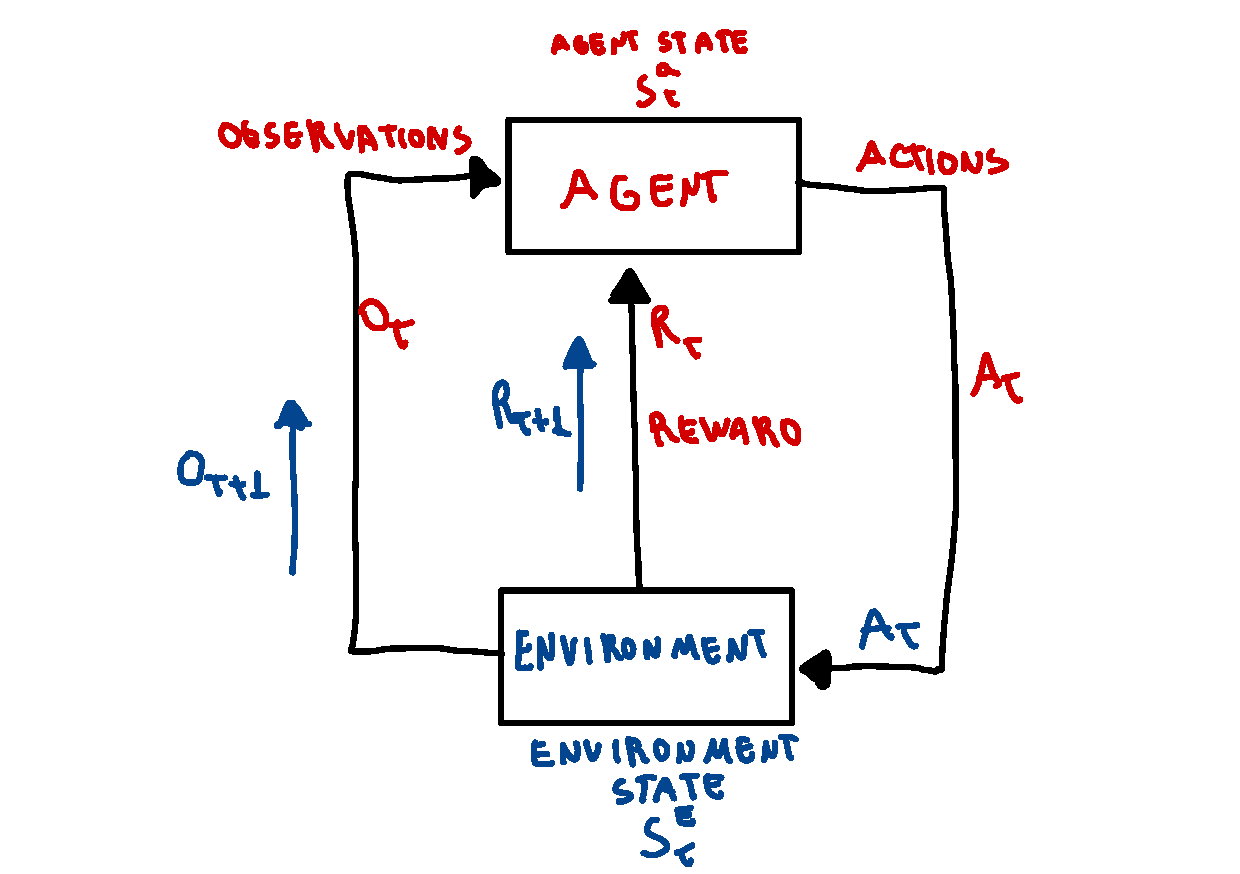
\includegraphics[width=0.9\textwidth]{sections/introduction/figures/reinforcement_learning_framework.pdf}
        \end{figure}
    \end{frame}

\end{frame}


\begin{frame}
    \frametitle{Agent and Environment}

    \begin{columns}
        % Column 1
        \begin{column}{0.5\textwidth}

            \begin{itemize}
                \item At each step $t$ the agent:

                \begin{itemize}
                    \item Execute action $A_t$;
                    \item Receives observation $O_t$;
                    \item Receives scalar reward $R_t$;
                \end{itemize}
           

                \item The enviroment
                
                \begin{itemize}
                    \item Receives action $A_t$;
                    \item Emits observation $O_{t+1}$;
                    \item Emits scalar reward $R_{t+1}$;
                \end{itemize}

                \item $t$ increments at enviroment step.

            \end{itemize}

        \end{column}


        % Column 2    
        \begin{column}{0.5\textwidth}
            \begin{figure}
            \centering
                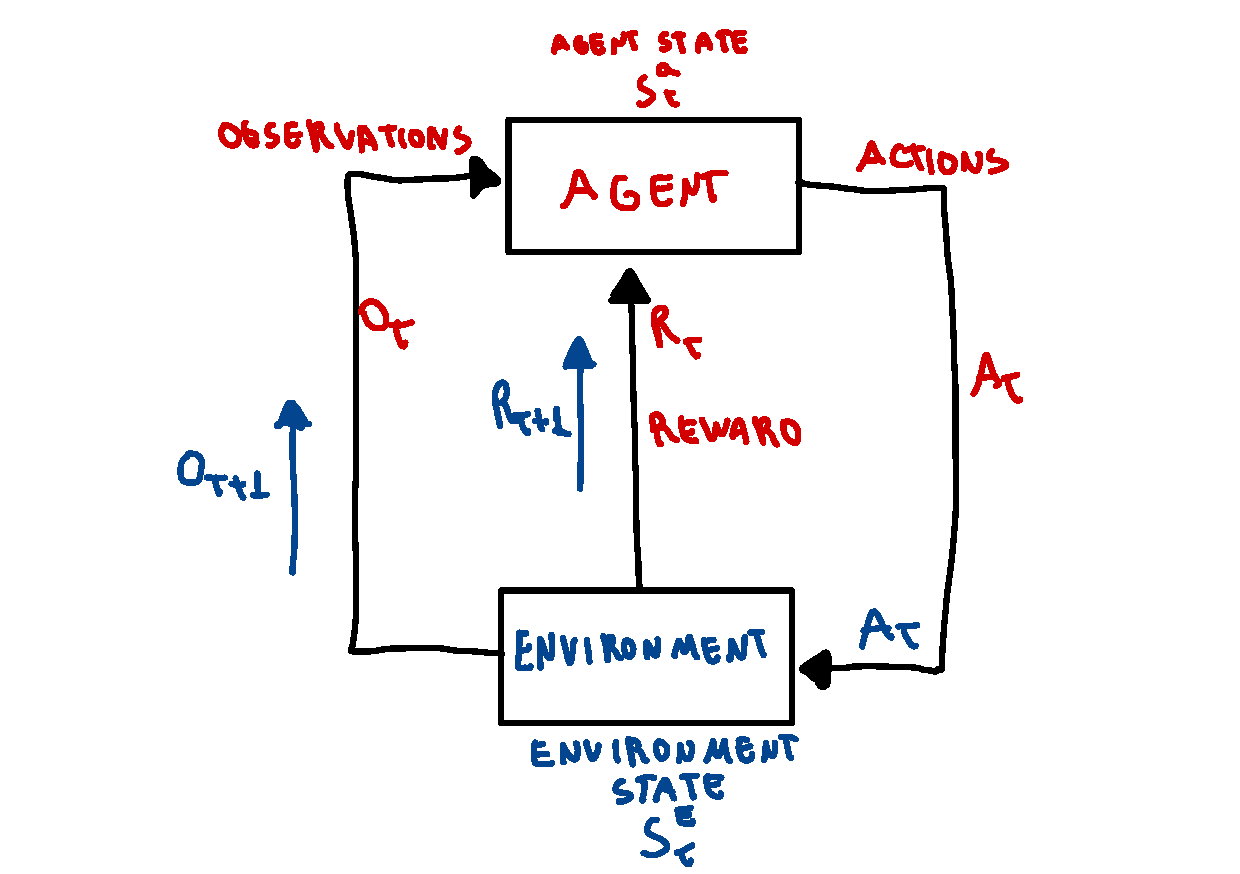
\includegraphics[width=1\textwidth]{sections/introduction/figures/reinforcement_learning_framework.pdf}
            \end{figure}
        \end{column}

    \end{columns}
\end{frame}






\begin{frame}

    \frametitle{Rewards}

    Reinforcement learning is based on the reward hypothesis.

    \begin{itemize}
        \item A reward $R_t$ is a scalar feedback;
        \item Indicates how well the agent is doing at step $t$ (reward depends on the context);
        \item The agent needs to maximise the cumulative reward.
    \end{itemize}

    \begin{definition}
        All goals can be described by the maximisation of expected cumulative reward.
    \end{definition}


\end{frame}


\begin{frame}
    \frametitle{Rewards (Examples)}

    \begin{itemize}
        \item Play many different Atari games better than humans:
        \begin{itemize}
            \item Positive reward for increasing the score
            \item Negative reward for decreasing the score;
        \end{itemize}

        \item Finacial problems:
        \begin{itemize}
            \item Positive reward for winning money;
            \item Negative reward for losing money;
        \end{itemize}

        \item Self-driving car:
        \begin{itemize}
            \item Positive reward for following desired trajectory;
            \item Negative reward for crashing the car;
        \end{itemize}
        
        \item Control a power station:
        \begin{itemize}
            \item Positive reward for producing energy;
            \item Negative reward for exceeding safety thresholds;
        \end{itemize}
    \end{itemize}

\end{frame}

\begin{frame}
    \frametitle{History and State}

    \begin{itemize}
        \item The history is the sequence of [observation, actions and rewards];
            $$H_t = [O_1,R_1,A_1], ..., [A_{t-1},R_t,R_t]$$
        \item What happens next depends on the history;
        \item State is the information used to determine what happens next;

        \item State is a function of the history:
            $$S_t = f(H_t)$$

        \item Should we use all history information to take the next action (move to the next state)?
    \end{itemize}

\end{frame}


\begin{frame}
    \frametitle{Agent and Environment State}


    \begin{itemize}
        \item The agent state $S^{a}_t$ is the agent's internal
        representation;

        \begin{itemize}
            \item Whatever information the agent uses to pick the next action;
            \item It can be any function of history:
            $$S^{a}_t = f(H_t)$$
        \end{itemize}

        \item The environment state $S^{e}_t$ is the environment's private
        representation:
        \begin{itemize}
            \item The environment state is not usually visible to the agent;
        \end{itemize}
   


    \end{itemize}
\end{frame}


\begin{frame}

    \frametitle{}

    \begin{columns}
        % Column 1
        \begin{column}{0.5\textwidth}
            Complete Observation:
            \begin{itemize}
                \item when the agent is able to observe the complete state 
                information that defines the status of the environment 
                after the agent has acted out a certain action, in it;

                \item Can be modeled as Markov Decision Process (MDP);
               
            \end{itemize}

        \end{column}

        % Column 2    
        \begin{column}{0.5\textwidth}
            Partial Observability:
            \begin{itemize}
                \item when the agent is able to observe only partial 
                information regarding the state of the environment;

                \item Partially observable problems can be converted indo MDPs.
               
            \end{itemize}
        \end{column}

    \end{columns}

\end{frame}



\begin{frame}

    Most part of problems in reinforcement learning are {\color{red}modeled as Markov chains}.
    An information state (a.k.a. Markov state, memoryless process) contains all useful information from the history.

    \begin{definition}
        A state $S_t$ is Markov if and only if 
        $$P[S_{t+1}|S_t] = P[S_{t+1}|S_t, S_{t-1},...,S_2,S_1]$$
    \end{definition}

    \begin{itemize}
        \item Once the state is knowm the entire history may be thrown away (not necessary to save all history);
        \item The future is independend of the past given the present;
        \item {\color{red}To move to the next state we only need to know the current state;}
        \item The history is Markov;

    \end{itemize}

\end{frame}



\begin{frame}
    \frametitle{Major Components of a RL Agent}

    An RL agent may include one or more of these components:
    \begin{itemize}
        \item Policy: agent's behaviour function;
        \begin{itemize}
            \item It is map from state to action;
            \item Deterministic policy $a = \pi(s)$:
            \item Stochastic policy: $\pi(a|s) = P[A_t=a|S_t=s]$
        \end{itemize}
        \item Value function: is a prediction of {\color{red}future reward}:
        \begin{itemize}
            \item Used to evaluate the goodness or badness of states;
            \item And to select between a set of actions given the current state;
            \item $v_{\pi}(s) = \E_{\pi}[R_{t+1}+\gamma~R\_{t+2}+\gamma^{2}R_{t+3}+...|S_t=s]$
        \end{itemize}   

        \item Model: predicts what the environment will do next

    \end{itemize}

\end{frame}


\begin{frame}
    \frametitle{Categorinzing RL agents}
    \begin{columns}
        % Column 1
        \begin{column}{0.5\textwidth}
            \begin{itemize}
                \item Model Free:
                \begin{itemize}
                    \item Policy and/or Value Function;
                \end{itemize}
                \item Model Based:
                \begin{itemize}
                    \item Policy and/or Value Function;
                    \item Model.
                \end{itemize}       
            \end{itemize}
        \end{column}

        % Column 2    
        \begin{column}{0.5\textwidth}
            \begin{itemize}
                \item Value Based;
                \item Policy Based;
                \item Actor Critic: Policy and Value Fucntions;
            \end{itemize}  
        \end{column}

    \end{columns}

\end{frame}